\chapter{对偶理论}\label{chap:duality}
\begingroup
\newcommand{\pref}{Chapters/duality/figures}


在本章中,我们考虑带约束的规划问题. 它的一般形式是
        \begin{alignat*}{2}
        \min\quad&f({x}) \\
        \text{s.t.}\quad&h_i({x})=0,&\quad i=1,\dots,m,\\
        &g_j(x)\leq 0,&\quad j=1,\dots,p,\\
        &x\in\Omega\subseteq\R^n.
        \end{alignat*}
其中,$m\le n$,函数$f,h_i,g_j$都是连续的,且通常假设它们拥有连续的二阶导. 

为简化记号,们用向量形式的函数,即${h}=(h_1,h_2,\dots,h_m)$和${g}=(g_1,g_2,\dots,g_p)$,把问题的形式重写为:
    \begin{align*}
        \min\quad& f({x}) \\
        \text{s.t.}\quad& {h}({x})={0},\\
        & {g}({x})\le {0}, \\
        & {x} \in \Omega.
    \end{align*}

约束${h}({x})={0},{g}({x})\le{0}$被称作\textbf{\index{函数约束}函数约束}. ${x}\in\Omega$是\textbf{\index{集合约束}集合约束}. 我们并不强调集合约束,因此假设在大部分情况下$\Omega$就是整个$\R^n$的空间,或者问题的解就在$\Omega$的内部. 

一个满足所有函数约束的点${x}\in\Omega$被称作\textbf{\index{可行解}可行解},而使得$f$取得最小值的可行解叫做\textbf{\index{最优解}最优解}. 有时候优化问题的目标可能是最大化$f$,此时相应的最优解就是使得$f$取得最大值的可行解. 本章的任务是讨论各种情况下最优值的必要条件,这些必要条件最终形成了所谓的\textbf{对偶理论}\index{对偶理论}. 

\section{条件极值与Lagrange乘子法}
我们现在先只考虑等式约束
\begin{equation}
\begin{aligned}
        \min\quad& f({x}) \\
        \text{s.t.}\quad& {h}({x})={0},\\
        & {x} \in \Omega.
\end{aligned}    \label{eq:eq-constraint-only-differentiable}
\end{equation}

这些约束定义了一个$\R^n$的子集,可以被看作一个曲面. 在恰当的条件下,这个曲面是$n-m$维的(类比线性空间). 如果函数$h_i,i=1,2,\dots,m$有一阶连续导数(记为属于$C^1$),那么他们定义的曲面就是\emph{光滑}\index{光滑曲面}的. 曲面上可以定义\emph{切空间}.
    
为了引入切空间,我们先介绍曲线,然后曲线的定义可以导出切空间的定义. 
\begin{definition}[曲线与切空间]\index{曲线}
\begin{itemize}
    \item 超平面$S$上的一条\textbf{曲线}是一系列点的集合:${x}(t)\in S$,它们以$t$为参数,$a\le t\le b$且在该区间上连续. 
    \item 称曲线是\textbf{可微的}\index{曲线!可微~},如果$\dot{{x}}=\d({x}(t))/\d t$存在. 
    \item 称曲线${x}(t)$\textbf{经过点${x^\ast}$},如果存在$t^\ast\in[a,b]$使得${x^\ast}={x}(t^\ast)$. 
    \item 曲线在${x^\ast}$的\textbf{导数}\index{曲线!~的导数}被定义为$\dot{{x}}(t^\ast)$,该导数是$\R^n$内的一个向量,这个向量可以看作沿着曲线$t$在$x^\ast$处的切向量.
    \item 考虑所有$S$内经过点${x^\ast}$的可微曲线. 点${x^\ast}$处的\textbf{切空间}\index{切空间}\,$T_{x^\ast}(S)$被定义为这些曲线在点${x^\ast}$处的导数的集合. 
\end{itemize}
\end{definition}

切空间的重要特点是,它是一个线性空间.
\begin{lemma}\label{lemma:tan-space}\index{线性空间}
    切空间是一个线性空间. 
\end{lemma}

既然切空间是一个线性空间,我们的一个主要目标就是给出切空间的显示表达,比如给出它的一组基向量. 考虑一条曲线$x(t)$,如果它在$h_i(x)=0$形成的曲面上,那么应该有
    \[\frac{\d}{\d t}h_i(x(t))=0\iff \nabla_x h_i(x(t))\dot{x}(t)=0.\]
因此${x}(t)$的切向量和该点处函数$h_i({x}(t))$的导数正交. 于是,如果$x(t)$在$h(x)=0$形成的曲面上,那么${x}(t)$处的导数$\nabla h(x(t))$是切平面的法向量. 这一数学推导的示意图见\Cref{fig:tangent-space}.

\begin{figure}
\centering
    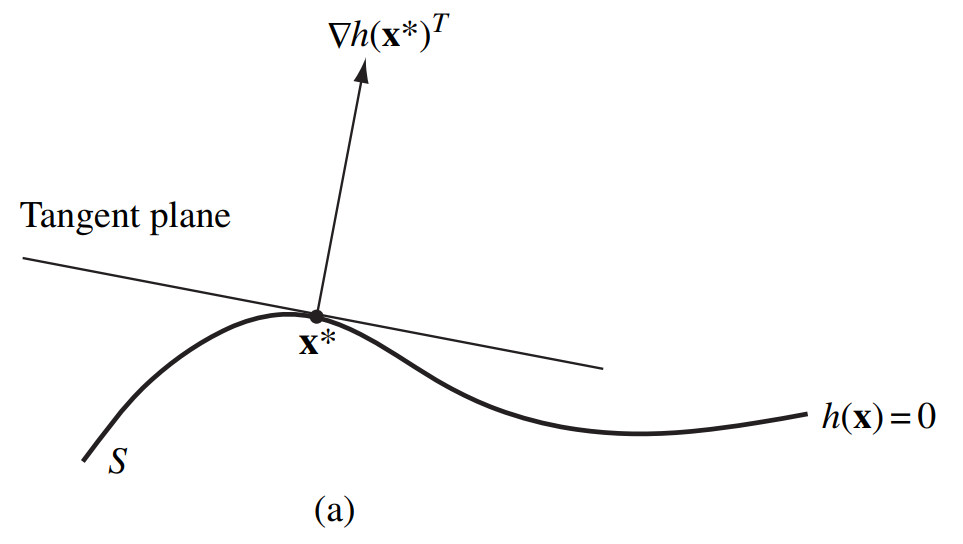
\includegraphics[scale=0.4]{\pref/tan-1dim.png}
\centering
    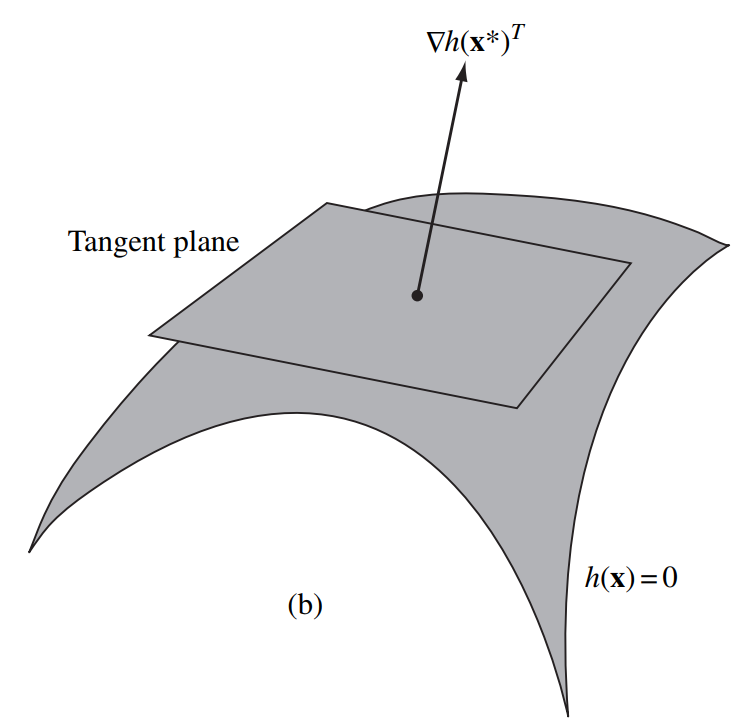
\includegraphics[scale=0.4]{\pref/tan-2dim.png}
\caption{切空间的示意图.}
\label{fig:tangent-space}
\end{figure}
    
我们把刚刚得到的垂直于$\nabla {h(x^\ast)y}$的子空间(即正交补空间)记作
    \[M=\{{y}\in\R^n:\nabla {h(x^\ast)y}=0\}.\]
我们已经证明$T_{x^\ast}(S)\subseteq M$. 反过来,在什么条件下会有$M=T_{x^\ast}(S)$?为此,我们引入\emph{正规点}的概念. 

\begin{definition}[正规点]\label{def:regular-point}\index{正规点}
考虑优化问题 \eqref{eq:eq-constraint-only-differentiable},当一个点${x^\ast}\in\Omega$满足约束${h(x^\ast)}=0$,且梯度向量$\nabla h_1({x^\ast}),\nabla h_2({x^\ast}),\dots,\nabla h_m({x^\ast})$线性无关时,它被称作该约束的\textbf{正规点}. 
\end{definition}

直观上来说,正规点上每一条约束都起到了实际的作用,因此梯度向量$\nabla h_i({x^\ast})$形成了一个线性无关的集合,张成了空间$M^\perp$. 此时,切空间恰好完全垂直于$M^\perp$,即$T_{x^\ast}(S)=M$. 这一几何直观见\Cref{fig:tan-2constraint},点${x^\ast }$处的两个等式约束共同确定了该点的切空间. 因此,在正规点,用约束函数的梯度来描述切空间是可行的. 
    \begin{figure}
        \centering
        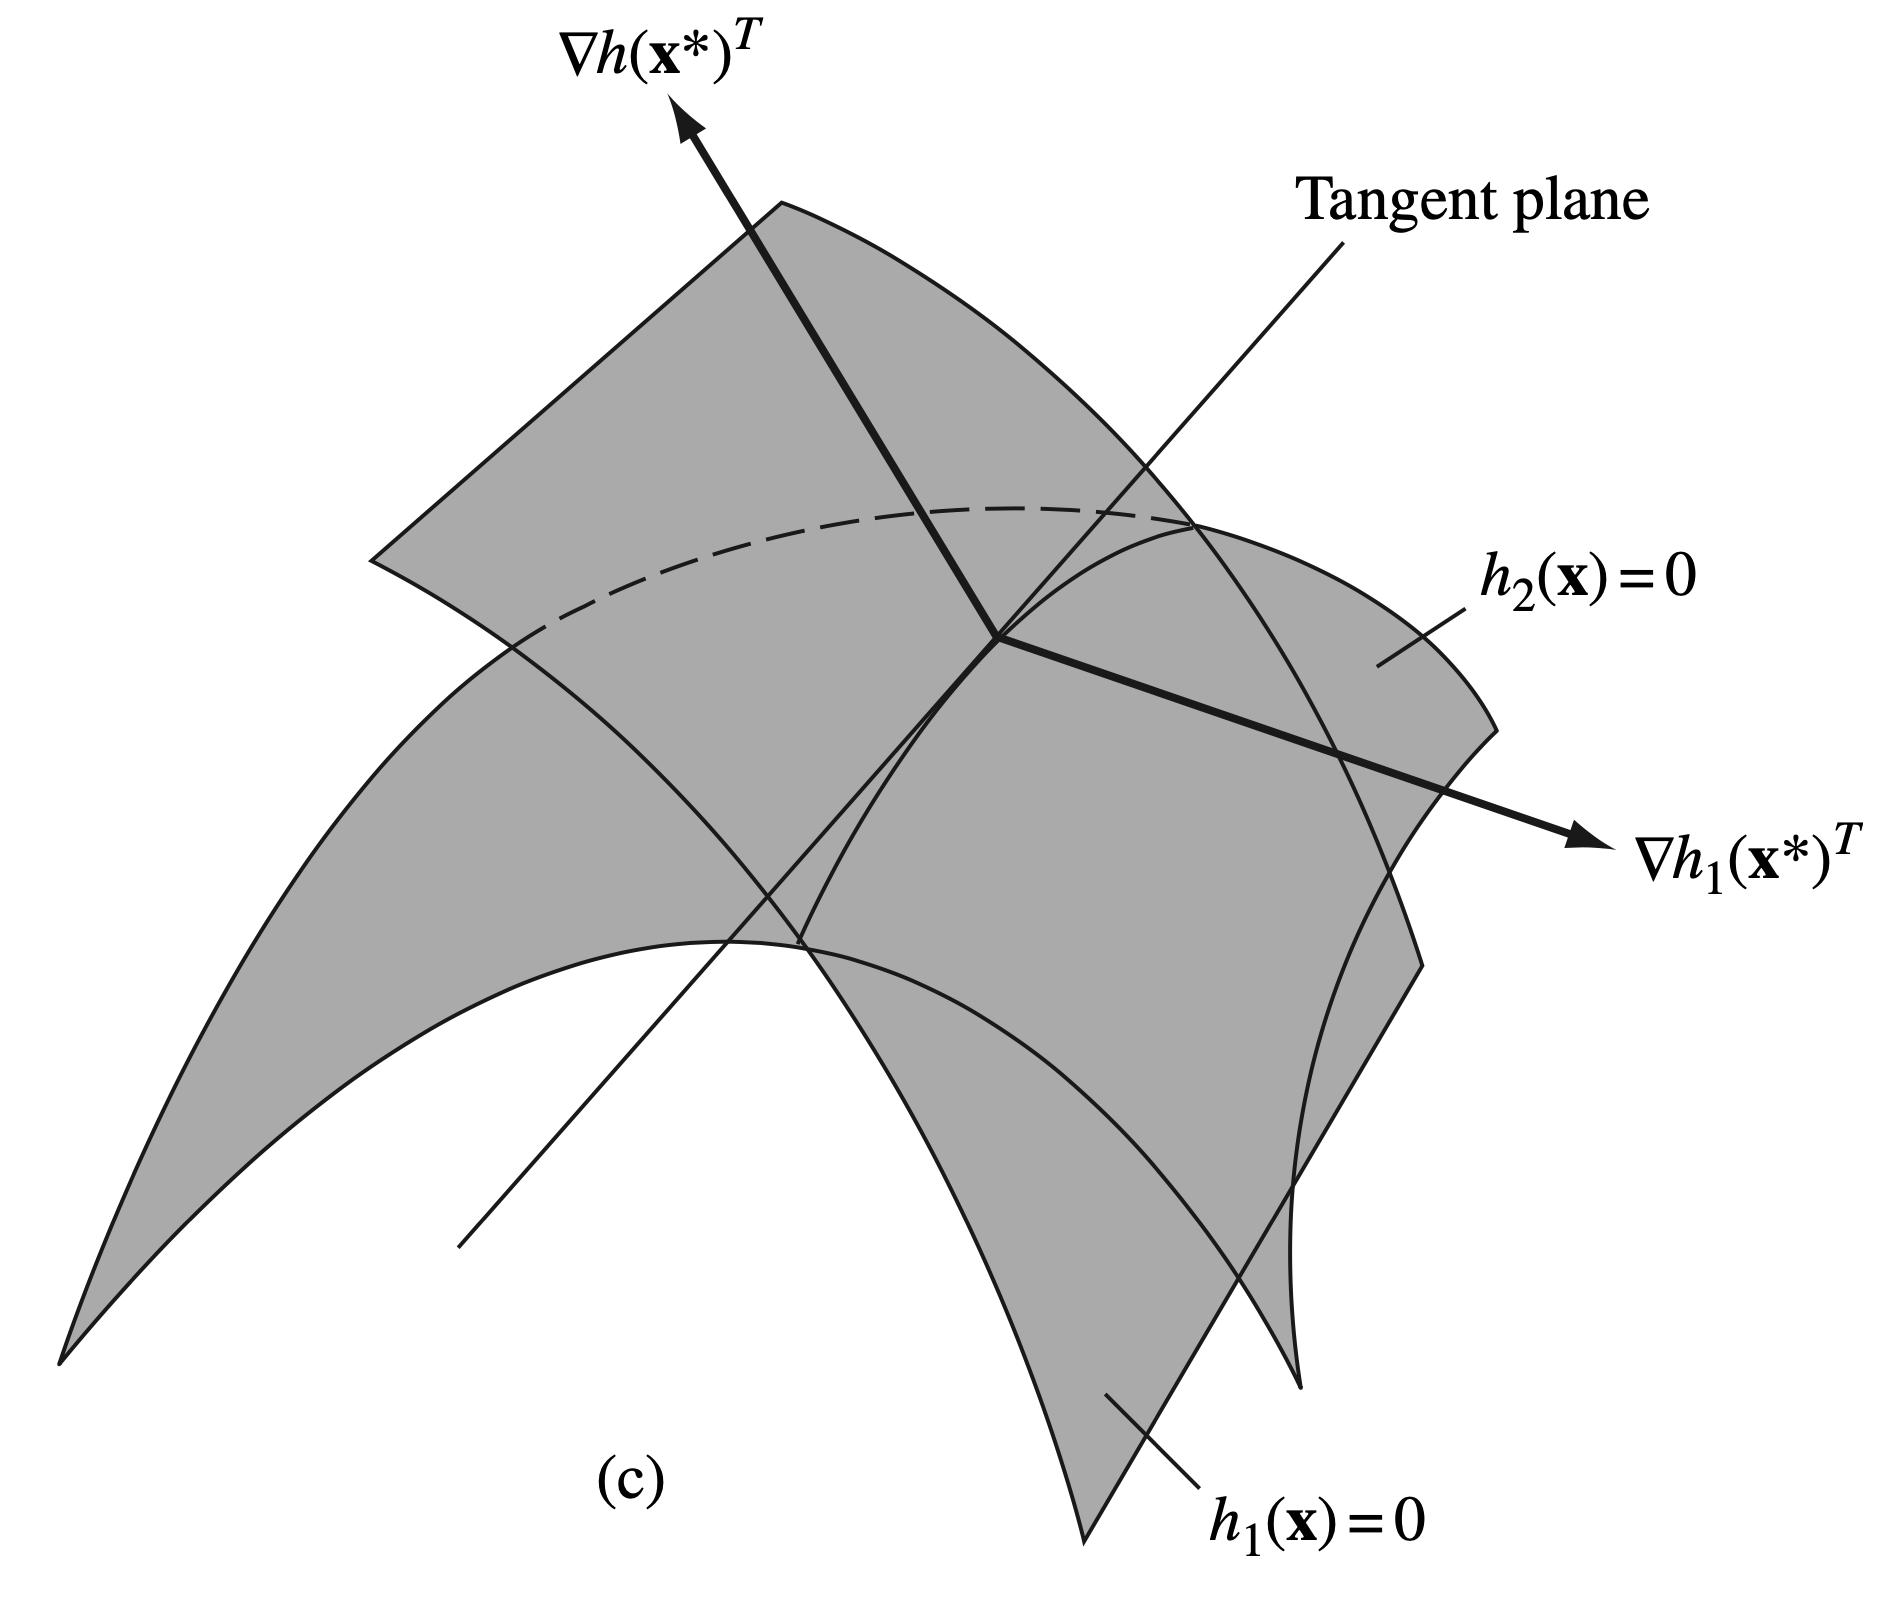
\includegraphics[scale=0.17]{\pref/tan-2constraint.png}
        \caption{正规点示意图. }
        \label{fig:tan-2constraint}
    \end{figure}

\begin{theorem}[正规点切空间刻画定理]
设曲面$S\subseteq\R^n$由约束$h(x)=0$定义,${x^\ast}\in S$是正规点,那么,
\[T_{x^\ast}(S)=M=\{{y:\nabla h(x^\ast)y=0}\}.\]
\end{theorem}
该定理的证明需要隐函数定理,对微积分要求较高,我们这里略去.

有了切空间的准备,现在我们要对正规点推导带约束的优化问题的极值条件. 考虑优化\eqref{eq:eq-constraint-only-differentiable},设$x^\ast$ 是一个约束${h(x)=0}$一个正规点,同时也是函数$f$的一个在可行域中的极值点.

\begin{lemma}\label{lemma:eq-opt-cond-1}
对$y\in\R^n$,如果$\nabla {h(x^\ast)y=0}$,那么$\nabla f({x^\ast}){y}=0$.
\end{lemma}

\begin{proof}
因为$x^\ast$是正规点,根据正规点切空间刻画定理,$\nabla h(x^*)y=0$等价于$y$是${x^\ast}$处的切空间中的向量. 根据定义,存在该约束曲面内的某个光滑曲线${x}(t)$,经过点${x^\ast}$,并且以$y$为切向量. 那么,${x}(0)={x^\ast}$,${\dot{x}}(0)={y}$,且${h(x(t))=0}$在区间$-a\le t\le a$上成立(对某个正数$a$). 因为点${x^\ast}$是一个函数$f$的受等式约束的极值点,我们有
\[\left.\frac{\d}{\d t}f({x}(t))\right|_{t=0}=0\iff \nabla f({x^\ast})y=0.\]
\end{proof}

\Cref{lemma:eq-opt-cond-1} 对任意$y\in\R^n$都成立,根据线性代数零空间的性质,这等价于$\nabla f(x^*)$是$\nabla h_i(x^*)$的线性组合,即
\[\nabla f(x^*)=\sum_i\lambda_i\nabla h_i(x^*).\]
据此,我们得到条件极值的一阶必要条件:
\begin{theorem}[条件极值的一阶必要条件]\label{thm:eq-opt-cond-1}\index{一阶必要条件}
    令${x^\ast}$是一个$f$的满足约束${h(x)=0}$的正规极值点. 那么存在一个${\lambda}\in \R^m$使得$$\nabla f({x^\ast})+{\lambda^\t \nabla h(x^\ast)=0}. $$
\end{theorem}

一阶必要条件$\nabla f({x^\ast})+{\lambda^\t}\nabla {h(x^\ast)=0}$以及约束${h(x^\ast)=0}$给出了$n+m$个等式,包含${x^\ast,\lambda}$在内的$n+m$个变量. 因此在非退化的情况下,他们给出了一个唯一解. 

引入与这个约束问题对应的Lagrange函数:
        $$l({x,\lambda})=f({x})+{\lambda^\t h(x)}.$$
$\lambda$被称为\emph{Lagrange乘子}\index{Lagrange乘子}. 必要条件可以被写作:
\begin{align*}
    \nabla_x l({x,\lambda})&=0,\\
    \nabla_{\lambda} l({x,\lambda})&=0.
\end{align*}


\begin{example}[最大熵]\label{ex:max-entropy}
考虑一个离散的概率分布,其分布列为$p_i=\Pr(X=x_i),i=1,\dots,n$. 该分布的熵为
$$\epsilon = -\sum_{i=1}^n p_i \log p_i.$$
该分布的均值为$\sum_{i=1}^n x_i p_i$. 

如果均值固定为$m$,求解使熵最大化的参数可以被转化成以下问题:
\begin{align*}
\max\quad&-\sum_{i=1}^n p_i\log p_i \\
\text{s.t.}\quad& \sum_{i=1}^n p_i=1, \\
&\sum_{i=1}^n x_i p_i=m, \\
&p_i\ge 0, \qquad i=1,2,\dots,n.
\end{align*}

我们先忽略非负约束,假设这些约束不会被触发. 引入两个Lagrange乘子,$\lambda$和$\mu$,则Lagrange函数为
$$l=\sum_{i=1}^n (-p_i\log p_i+\lambda p_i+\mu x_ip_i)-\lambda-\mu m.$$
由一阶必要条件,$-\log p_i -1+\lambda+\mu x_i=0$,$i=1,2,\dots,n$. 因此,
$$p_i=\exp((\lambda-1)+\mu x_i),\quad i=1,2,\dots, n.$$
注意$p_i>0$,所以非负约束确实没有被触发. Lagrange乘子$\lambda$和$\mu$是两个用来保证等式约束被满足的参数. 
\end{example}

\section{Karush–Kuhn–Tucker条件}
现在加入不等式约束,考虑以下形式的问题:
\begin{equation}
\begin{aligned}
\min\quad& f({x}) \\
\text{s.t.}\quad& {h(x)=0}, \\
&{g(x)\le0}. 
\end{aligned}\label{eq:ineq-constraint-inequality-differentiable}
\end{equation}
假设$f$和${h}$和前面一样,${g}$是一个$p$维的函数,$f,{h,g}\in C^1$. 

我们推广正规点$x^\ast$的定义为:
\begin{definition}[正规点]\index{正规点}
考虑优化问题 \eqref{eq:ineq-constraint-inequality-differentiable},点$x^\ast$被称为\textbf{正规点},如果
\begin{itemize}
    \item 它满足约束:$h(x^\ast)=0, g(x^\ast)\le 0$.
    \item 令$J$为满足$g_j({x^\ast})=0$的下标$j$的集合(激活的约束). 那么,梯度向量$\nabla h_i({x^\ast})$,$\nabla g_j({x^\ast})$,$1\le i \le m$,$j\in J$是线性无关的.
\end{itemize}
\end{definition}

换言之,此时的正规点不仅考虑等式约束,还要考虑起作用的或者说被激活的不等式约束,这些不等式约束相当于等式约束. 类似Lagrange乘子法,此时的一阶必要条件为:

\begin{theorem}[Karush-Kuhn-Tucker条件]\label{thm:KKT}\index{Karush-Kuhn-Tucker条件}\index{一阶必要条件}
令${x^\ast}$为优化问题 \eqref{eq:ineq-constraint-inequality-differentiable} 的正规极小值点,那么,存在向量${\lambda}\in\R^m$和向量${\mu}\in \R^p$且${\mu\ge 0}$使得
\begin{align}
    \nabla f({x^\ast})+\lambda^\t \nabla {h(x^\ast)}+{\mu}^\t \nabla {g(x^\ast)}&={0},\label{eq:KKT-1}\\
    {\mu^\t g(x^\ast)}&=0.\label{eq:KKT-2}
\end{align}
\end{theorem}

\begin{proof}
首先,因为${\mu\ge 0}$且${g(x^\ast)\le 0}$,\eqref{eq:KKT-2} 等价于:${\mu}$的一个分量非零仅当对应的约束被激活(即取到等号). 这是一个互补松弛条件,即${g(x^\ast)}_i<0$可得出$\mu_i=0$,以及$\mu_i>0$可得出${g(x^\ast)}_i=0.$

设被激活的下标为$J$. 因为${x^\ast}$是约束集合上的一个极小点,它也是满足等式约束$h(x)=0,g_i(x)=0,i\in J$的极小点. 因此,在新的等式约束问题中,${x^\ast}$的邻域中存在Lagrange乘子,满足一阶必要条件. 我们得出结论:一阶必要条件 \eqref{eq:KKT-1} 成立,且若$g_j({x^\ast})\neq0$,则$\mu_j=0$.(于是也有 \eqref{eq:KKT-2} 成立)

现在还需要证明${\mu \ge 0}$. 用反证法,假设$\mu_k<0$对某个$k\in J$成立. 设$S$为其他所有被激活的约束在${x^\ast}$处定义的曲面,$M=T_{x^\ast}(S)$. 因为$x^\ast$是正规的,存在${y}\in M$且$\nabla g_k({x^\ast})y<0$. 令${x}(t)$为一条在$S$内且经过${x^\ast}$(此处$t=0$)的曲线,且有$\dot{{x}}(0)={y}$. 则对于充分小的$t\ge 0$,${x}(t)$是可行的,由 \eqref{eq:KKT-1} 以及$y\in M$,
\begin{align*}
    \left.\frac{\d f({x}(t))}{\d t}\right|_{t=0}=&\nabla f({x^\ast})y\\
    =&-\lambda^\t \nabla {h(x^\ast)}y-{\mu}^\t \nabla {g(x^\ast)}y\\
    =&-\mu_k\nabla g_k({x^\ast})y<0. 
\end{align*}
这与${x^\ast}$是极小点矛盾. 
\end{proof}

\begin{remark}
这一证明具有很强的几何直观,关键在于找一个可行的方向使得函数值下降. 非常需要注意的是,这一证明并不能用于否证$\mu_k>0$. 此时需要取${y}\in M$使得$\nabla g_k({x^\ast})y>0$. 然而此时对应的$x(t)$不再可行,因为对充分小的$t>0$,$g_k(x(t))>0$,违背了约束的条件.
\end{remark}

下面我们来看一个运用KKT条件的例子:
\begin{example}
考虑问题
\begin{align*}
    \min \quad &2x_1^2+2x_1x_2+x_2^2-10x_1-10x_2 \\
    \text{s.t.}\quad &x_1^2+x_2^2\le 5, \\
    & 3x_1+x_2\le 6.
\end{align*}
KKT条件为(注意,一阶必要条件还需要加入问题中的约束条件)
\begin{align*}
    4x_1+2x_2-10+2\mu_1x_1+3\mu_2&=0, \\
    2x_1+2x_2-10+2\mu_1x_2+\mu_2&=0, \\
    \mu_1(x_1^2+x_2^2-5)&=0, \\
    \mu_2(3x_1+x_2-6)&=0,\\
    \mu_i&\ge 0,\quad i=1,2.
\end{align*}
为了求解此类问题,我们假设一些约束被激活,然后检查所得出的Lagrange乘子的符号正负. 在这个问题中,我们可以尝试假设有0,1,2个约束被激活. 

假设第一个约束被激活,第二个约束没有被激活,得出等式
\begin{align*}
4x_1+2x_2-10+2\mu_1x_1&=0, \\
2x_1+2x_2-10+2\mu_1x_2&=0, \\
x_1^2+x_2^2&=5.
\end{align*}
可得解$x_1=1,x_2=2,\mu_1=1.$

由于$3x_1+x_2=5$,因此第二个约束也被满足了. 因此,因为$\mu_1 > 0$,我们得出结论,这个解满足一阶必要条件. 
\end{example}

\section{Lagrange对偶}
\subsection{Lagrange定理}
现在,我们不再假设函数可微,我们考虑极值点的零阶必要条件\index{零阶必要条件},首先考虑只有等式约束的情形:
    \begin{equation}
          \begin{aligned}
        \min&\quad f({x}) \\
        \text{s.t.}\quad& {h(x)=0}, \\
        &{x}\in\Omega.
        \end{aligned}\label{eq:eq-zero-cond}
    \end{equation}
如果函数$f$是凸函数,$m$维函数${h}$是仿射的,并且集合$\Omega\subset \R^n$是是凸的,那么这个规划问题是一个\emph{凸规划问题}\index{凸规划问题}. 

为了给这样的问题一个一阶必要条件,我们依然需要引入正规性条件. 此时正规性不再仅仅只对一个点,而是对仿射函数$h$.

\begin{definition}[正规性条件]\index{正规性条件}
一个仿射函数${h}$关于集合$\Omega$是\textbf{正规的},指的是像集$h(\Omega)=\{y:\exists x\in\Omega\ h(x)=y\}$包含${0}$处的一个开球邻域. 也就是说,$h(\Omega)$包含一个形如$\{y:\norm{y}<\epsilon\}$(对某个$\epsilon>0$)的集合. 
\end{definition}

\begin{remark}
这个条件是一阶正规点定义的推广. 如果${h}$在点${x^\ast}$有连续的导数,那么一阶正规性条件意味着$\nabla{h(x^\ast)}$是满秩的,并且由隐函数定理可知存在一个$\epsilon>0$使得对于任意满足${\norm{y-h(x^\ast)}}<\epsilon$的${y}$,都有一个${x}$使得${h(x)=y}$. 换言之,存在一个${y^\ast=h(x^\ast)}$周围的开球.
\end{remark}

我们可以用Lagrange乘子来表述零阶必要条件:
\begin{theorem}[零阶必要条件,等式约束情形]\label{thm:eq-zero-cond}\index{零阶必要条件}
假设$\Omega\subset\R^n$是凸的,$f$是$\Omega$上的凸函数,${h}$是一个$\Omega$上的$m$维仿射函数. 假设${h}$是对于$\Omega$正规的. 如果${x^\ast}$是 \eqref{eq:eq-zero-cond} 的解,那么存在${\lambda}\in \R^m$使得${x^\ast}$是以下Lagrange问题的解:\begin{align*}
    \min\quad& f({x})+{\lambda^\t h(x)}\\
    \text{s.t.}\quad & x\in\Omega.
\end{align*}
\end{theorem}

这一定理证明的关键在于引入\emph{原始函数}. 对应于问题\eqref{eq:eq-zero-cond} 的\textbf{原始函数}\index{原始函数}是:$$\omega({y})=\inf\{f({x}):{h(x)=y,x}\in\Omega\},\quad y\in h(\Omega).$$


\begin{proof}[零阶必要条件的证明]
令$f^\ast=f({x^\ast})$. 定义$\R^m\times\R$内的集合$A$和$B$为:
\begin{align*}
    A&=\{(y,r):r\ge \omega({y}),{y}\in h(\Omega)\},\\ 
    B&=\{(y,r):r\le f^\ast,y=0\}.
\end{align*}
$A$是$\omega$的上图,$B$是$f^\ast$向下延申并与原点对齐的垂线. $A$和$B$都是凸集. 他们唯一的公共点是$(0,f^\ast)$. 由超平面分离定理可知,存在一个超平面分离$A$和$B$. 这个超平面可以被表示成一个在$\R^m\times\R$内的形如$(\lambda,s),\lambda\in \R^{m}$的非零向量,还有一个分离常数$c$. 分离条件是$$sr+{\lambda^\t y}\ge c,\quad\forall(y,r)\in A,\quad sr+{\lambda^\t y}\le c,\quad\forall(y,r)\in B.$$ 
这一过程的示意图见\Cref{fig:sep-hyperplane-eq}.

\begin{figure}[ht]
    \centering
    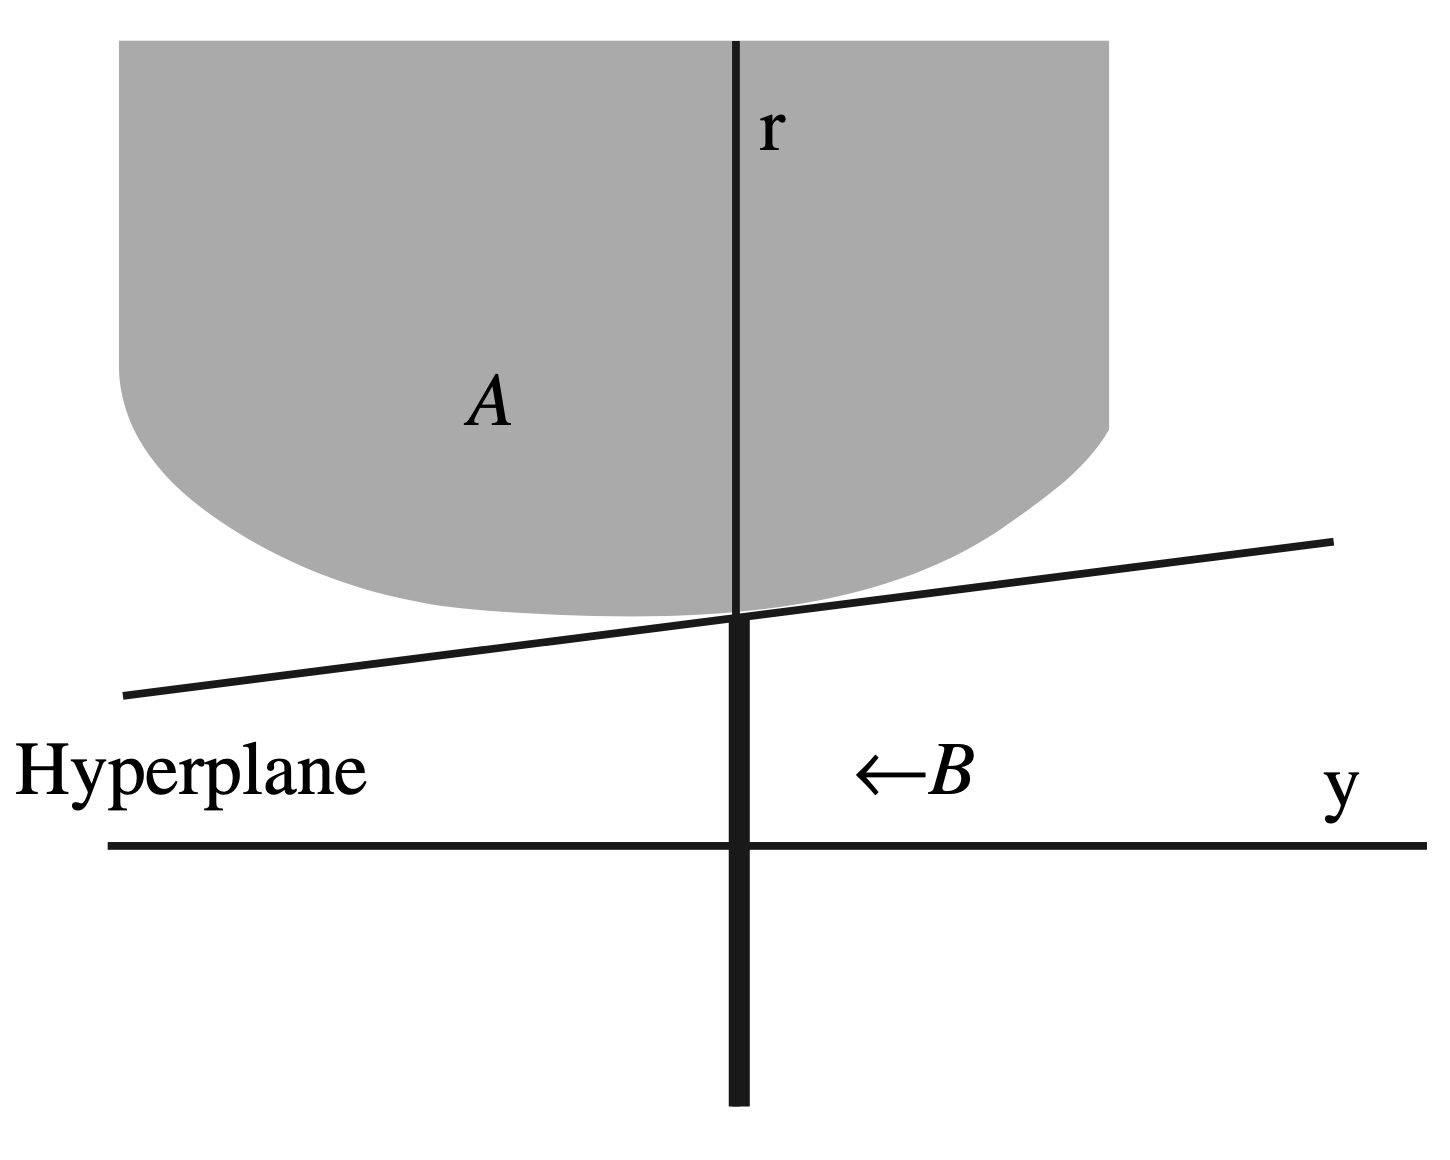
\includegraphics[scale=0.3]{\pref/sep-hyperplane-eq.png}
    \caption{证明示意图. }
    \label{fig:sep-hyperplane-eq}
\end{figure}

注意到$s\ge 0$,否则取$|r|$非常大的负数$r$,点$(r,{0})\in B$违反第二个分离不等式. 几何上看,若$s=0$,超平面将垂直. 我们来证明$s\neq 0$. 假设$s=0$,因为$s$和${\lambda}$不能都是$0$,${\lambda\neq 0}$. 因为分离超平面必须包含点$(f^\ast,{0})$,从第二个分离不等式得$c=0$. 由$h$的正规性,以${0\in h(\Omega)}$为中心的某个球包含在$h(\Omega)$中,任取$y$属于这个开球. 第一个分离不等式左侧为${\lambda^\t y}$,它对于某些${y}$来说是负的. 这违背第一个分离不等式. 因此$s\neq 0$,继而$s>0$. 

不失一般性,可以假设$s=1$. 假设$x\in\Omega$. 那么$(h(x),f(x))\in A$且$(0,f(x^\ast))\in B$. 因此,由分离不等式可知,我们有$$f({x})+{\lambda^\t h(x)}\ge f({x^\ast})=f({x^\ast})+{\lambda^\t h(x^\ast)}.$$ 因此${x^\ast}$是优化问题 \eqref{eq:eq-zero-cond} 解. 
\end{proof}

我们再考虑只有不等式约束的模型
\begin{equation}
    \begin{aligned}
    \min\quad & f({x})\\
    \text{s.t.}\quad& {g(x)\le 0},\\
    &{x}\in\Omega.
\end{aligned}\label{eq:ineq-zero-cond}
\end{equation}
其中,${g}$是一个$p$维的函数. 


然后我们引入正规性条件. 对于不等式约束来说,正规性条件也被称为做\emph{Slater条件}. 

\begin{definition}[Slater条件]\index{正规性条件}\index{Slater条件}
考虑优化问题 \eqref{eq:ineq-zero-cond},令
\[D=\{z\in \R^p:\exists x\in\Omega\ {g(x)\le z}\}.\]
正规性条件(Slater条件)为:存在一个$z^\prime\in D$使得$z^\prime<0$. 
\end{definition}
直观来说,Slater条件指的是存在满足约束的内点.

类似地,我们可以用Lagrange乘子来表述零阶必要条件:
\begin{theorem}[零阶必要条件,不等式情形]\label{thm:ineq-zero-cond}\index{零阶必要条件}
假设$\Omega$是一个$\R^n$的凸子集,且$f$和${g}$是凸函数. 假设优化问题 \eqref{eq:ineq-zero-cond} 满足正规性条件,${x^\ast}$是该问题的解,那么存在一个向量${\mu}\in \R^p$满足$\mu\ge 0$使得${x^\ast}$是下述Lagrange问题的解:
\begin{align*}
\min\quad &f({x^\ast})+\mu^\t g(x)\\
\text{s.t.}\quad& x\in\Omega.
\end{align*}
此外,${\mu^\t g(x^\ast)}=0.$
\end{theorem}

这一定理的证明类似于\Cref{thm:eq-zero-cond} 的证明. 首先还是引入原始函数. 问题 \eqref{eq:ineq-zero-cond} 对应的原始函数\index{原始函数}为:
    $$\omega({z})=\inf\{f({x}):g(x)\le{z},x\in\Omega\},z\in D.$$


\begin{proof}[证明概要]
令$f^\ast=f({x^\ast})$. 在$\R^{p}\times\R$内定义两个集合
\begin{align*}
    A&=\{(z,r):r\ge \omega(z), z\in D\},\\
    B&=\{(z,r):r\le f^\ast, z\leq 0\}.
\end{align*}
$A$和$B$都是凸的. 证明依然是构造$A,B$的分离超平面,正规性条件保证了超平面不会是垂直的. 这个过程的示意见图\Cref{fig:sep-hyperplane-ineq}.
\begin{figure}
    \centering
    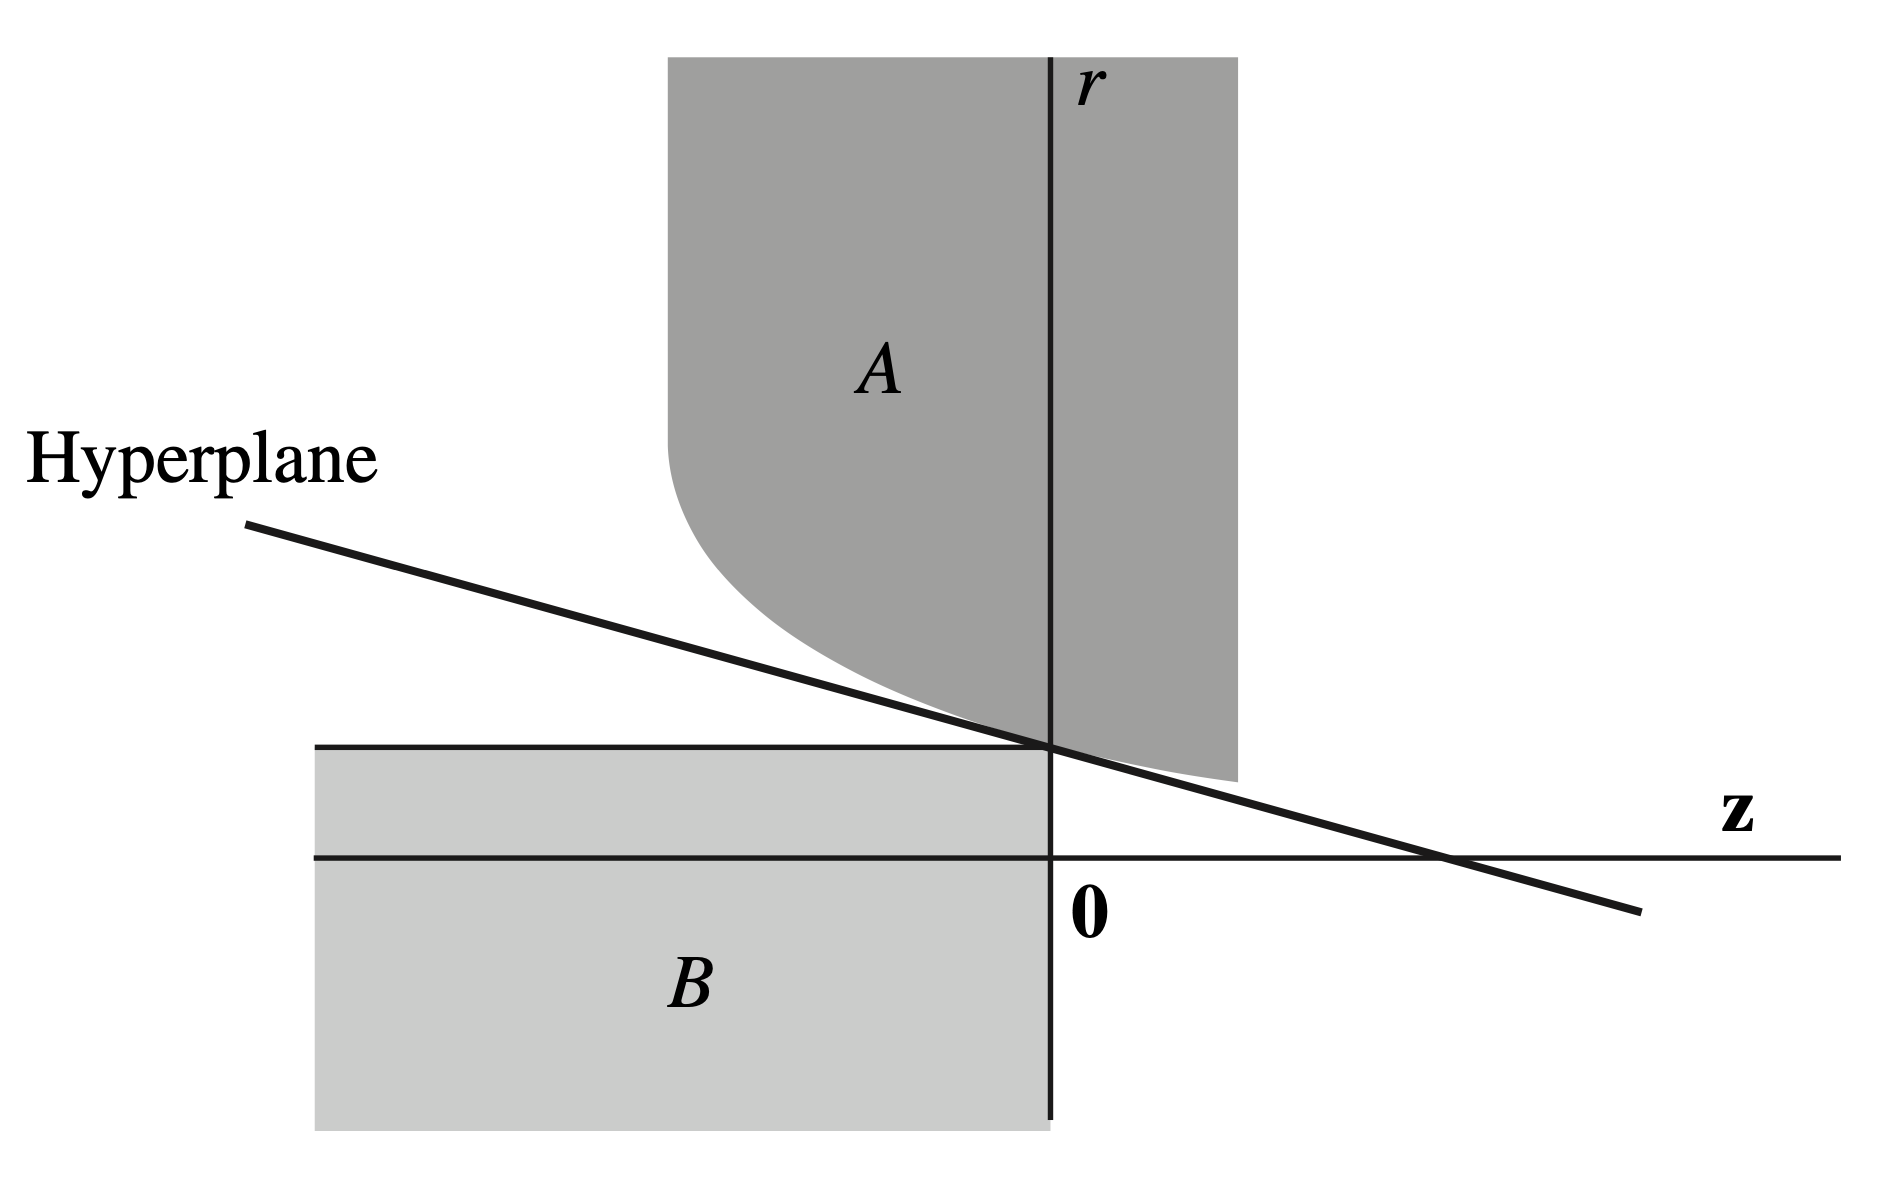
\includegraphics[scale=0.3]{\pref/sep-hyperplane-ineq.png}
    \caption{证明示意图. }
    \label{fig:sep-hyperplane-ineq}
\end{figure}

条件$\mu^\t g(x^\ast)=0$是互补松弛条件,这一讨论类似KKT条件. 
\end{proof}

现在,我们考虑一般情形,
    \begin{equation}
          \begin{aligned}
        \min\quad & f({x}) \\
        \text{s.t.}\quad& {h(x)=0}, \\
        &g(x)\leq 0, \\
        &{x}\in\Omega.
        \end{aligned}\label{eq:mix-zero-cond}
    \end{equation}
组合以上两个零阶必要条件,我们得到一般情形的Lagrange定理.

\begin{theorem}[Lagrange,零阶必要条件,混合情形]\label{thm:mix-zero-cond}\index{零阶必要条件}\index{Lagrange定理}
假设$\Omega\subset \R^n$是凸集. $f$和${g}$是一维和$p$维的凸函数,${h}$是维数为$m$的仿射函数. 假设${h}$满足对于$\Omega$的正规性条件,且$g$在 \eqref{eq:mix-zero-cond} 的可行域上满足正规性条件. 假设${x^\ast}$是问题 \eqref{eq:mix-zero-cond} 的解. 那么存在向量${\lambda}\in \R^m$和${\mu}\in \R^p$满足${\mu}\ge {0}$使得${x^\ast}$是以下Lagrange问题的解:
\begin{align*}
\min\quad &f({x})+\lambda^\t h(x)+\mu^\t g(x) \\
\text{s.t.}\quad& x\in\Omega.
\end{align*}
此外,${\mu^\t g(x^\ast)}=0.$
\end{theorem}

\lhysays{举个例子}


\subsection{弱对偶定理,强对偶定理}
Lagrange定理有非常强的几何直观,这一直观最终导致了优化中的\emph{对偶理论}\index{对偶理论}. 先考虑不等式约束的情形:
\begin{equation}
    \begin{aligned}
    \min\quad & f({x})\\
    \text{s.t.}\quad& {g(x)\le 0},\\
    &{x}\in\Omega.
\end{aligned}\label{eq:ineq-dual}
\end{equation}
$\Omega\subset \R^n$是凸集,函数$f$和${g}$定义在$\Omega$上. 函数${g}$是$p$维的. 

回忆原始函数的定义:
        $$\omega({z})=\inf \{f({x}):g(x)\le z,x\in\Omega\}.$$

设$x^\ast$是 \eqref{eq:ineq-dual} 的解,$f^\ast=f(x^\ast)$,那么函数$\omega(z)$与纵轴的交点是$f^*$. 如果 \eqref{eq:ineq-dual} 没有解,那么$f^*=\inf\{f(x):g(x)\leq 0,x\in\Omega\}$就是纵轴与$\omega(z)$的交点. 考虑在$\omega(z)$以下的超平面,关注其纵截距(见图\Cref{fig:hyperplane-below}),我们用它产生对偶原理.
\begin{figure}
    \centering
    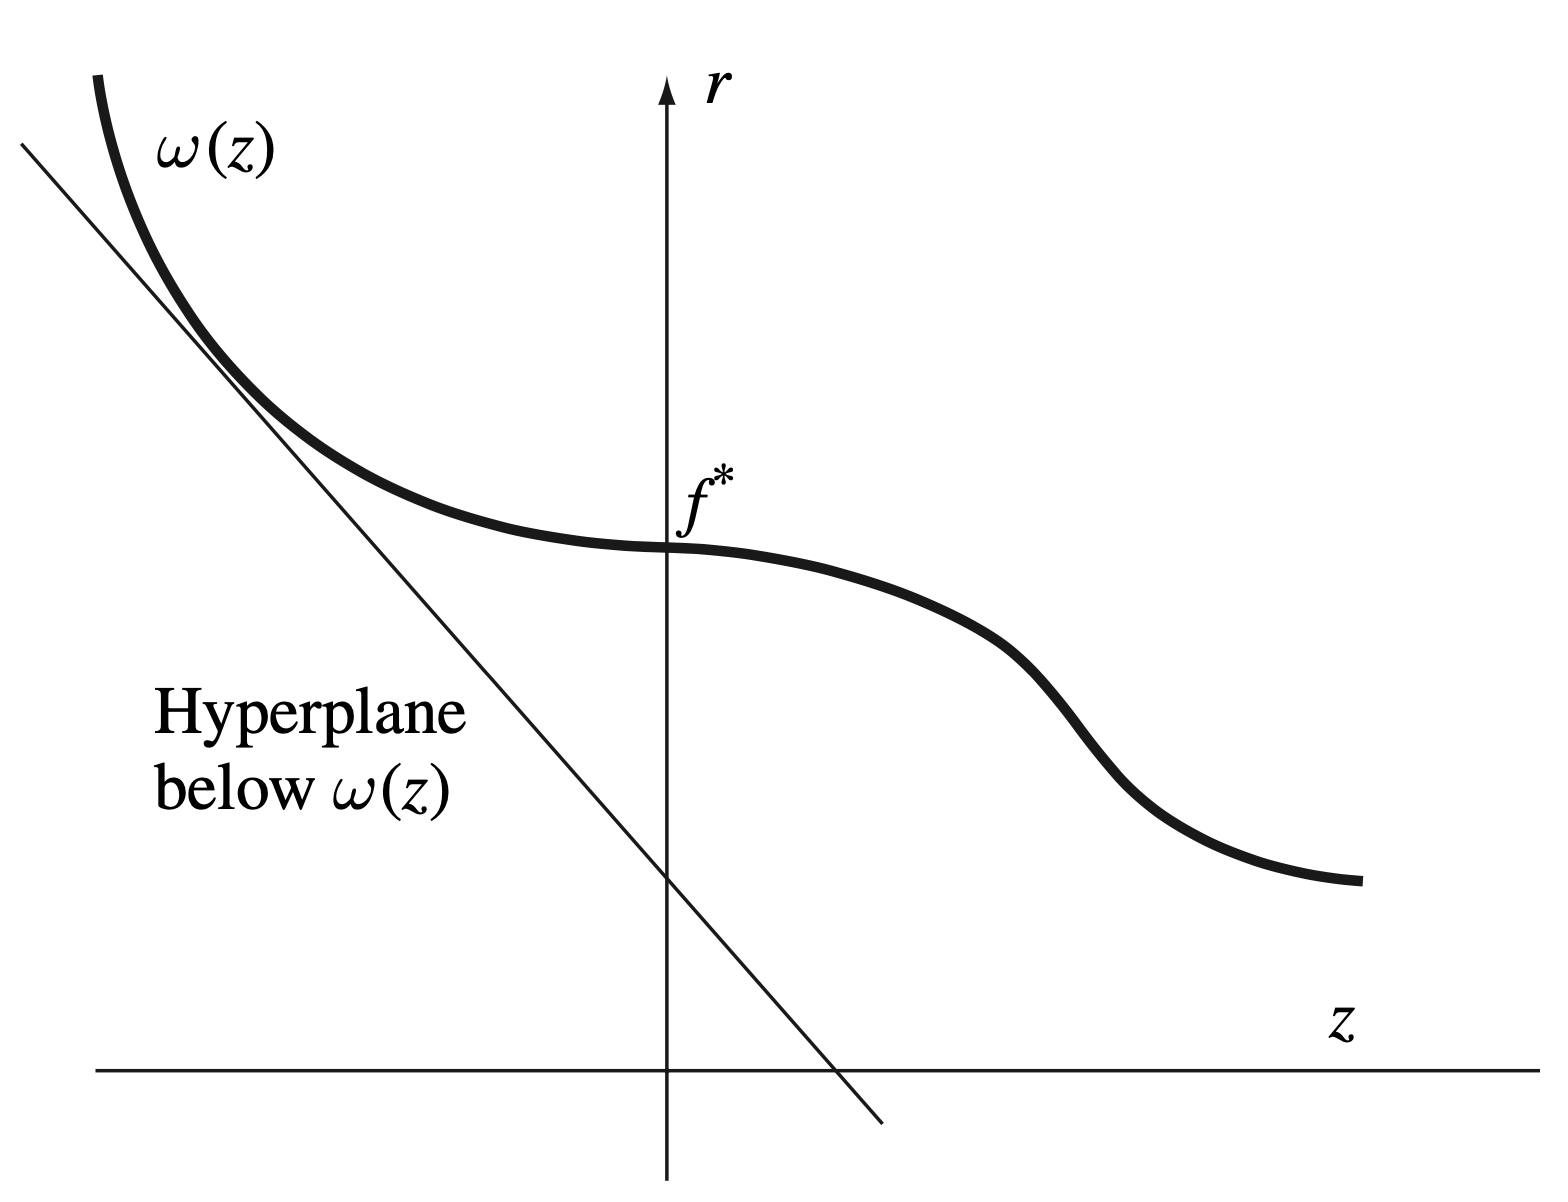
\includegraphics[scale=0.2]{\pref/hyperplane-below.png}
    \caption{纵截距的示意图.}
    \label{fig:hyperplane-below}
\end{figure}

为了刻画超平面以及其纵截距,我们引入对偶函数. 在$\R^p_{\geq 0}$上定义\textbf{对偶函数}\index{对偶函数}为:
$$\varphi({\mu})=\inf \{f({x})+{\mu^\t g(x)}:{x}\in\Omega\}.$$
定义其最大值为
    \[\varphi^*=\sup\{\varphi(\mu),\mu\geq 0\}.\]

我们很容易可以证明以下定理:

\begin{theorem}[弱对偶定理]\label{thm:weak-dual}\index{弱对偶定理}
    $\varphi^\ast\le f^\ast$.
\end{theorem}

\begin{proof}
    对任意${\mu \ge 0}$我们有
    \begin{align*}
        \varphi({\mu}) &=\inf\{f({x})+{\mu^\t g(x):x}\in\Omega\} \\
        & \le \inf\{f({x})+{\mu^\t g(x):g(x)\le 0,x}\in\Omega\} \\
        & \le \inf\{f({x}):{g(x)\le 0, x}\in\Omega\}=f^\ast.
    \end{align*}
    由此,$\varphi^\ast\le f^\ast$. 
\end{proof}

弱对偶定理也有非常几何的解释. 考虑向量$(\mu,1)\in \R^{p}\times\R$,${\mu}\ge{0}$和一个常数$c$. 关于$(z,r)$的方程$({\mu},1)^\t (z,r)=r+{\mu^\t z}=c$定义了一个$\R^{p}\times\R$内的超平面. 不同的$c$得到不同的超平面,他们都是平行的. 对于给定的$({\mu},1)$(即平行的超平面),选取一个最低的超平面,使得它刚刚碰到了原始函数上图边界. 假设${x_1}$是这个触点,有$r=f(x_1)$和$z=g(x_1)$. 那么$c=f({x_1})+{\mu^\t g(x_1)}=\varphi({\mu})$. 注意到此时$c=\varphi({\mu})$就是截距,这就是$\varphi(\mu)$的几何含义.

另一方面,求截距$c$(对偶函数值)的最大值$\varphi^*$,就是求位于原始函数之下的超平面的最大截距. 因此至少有$\varphi^*\leq f^*$,差$f^*-\varphi^*$被称为\emph{对偶间距}\index{对偶间距}. 这就是弱对偶定理,图示参见\Cref{fig:highest-hyperplane}.

\begin{figure}
    \centering
    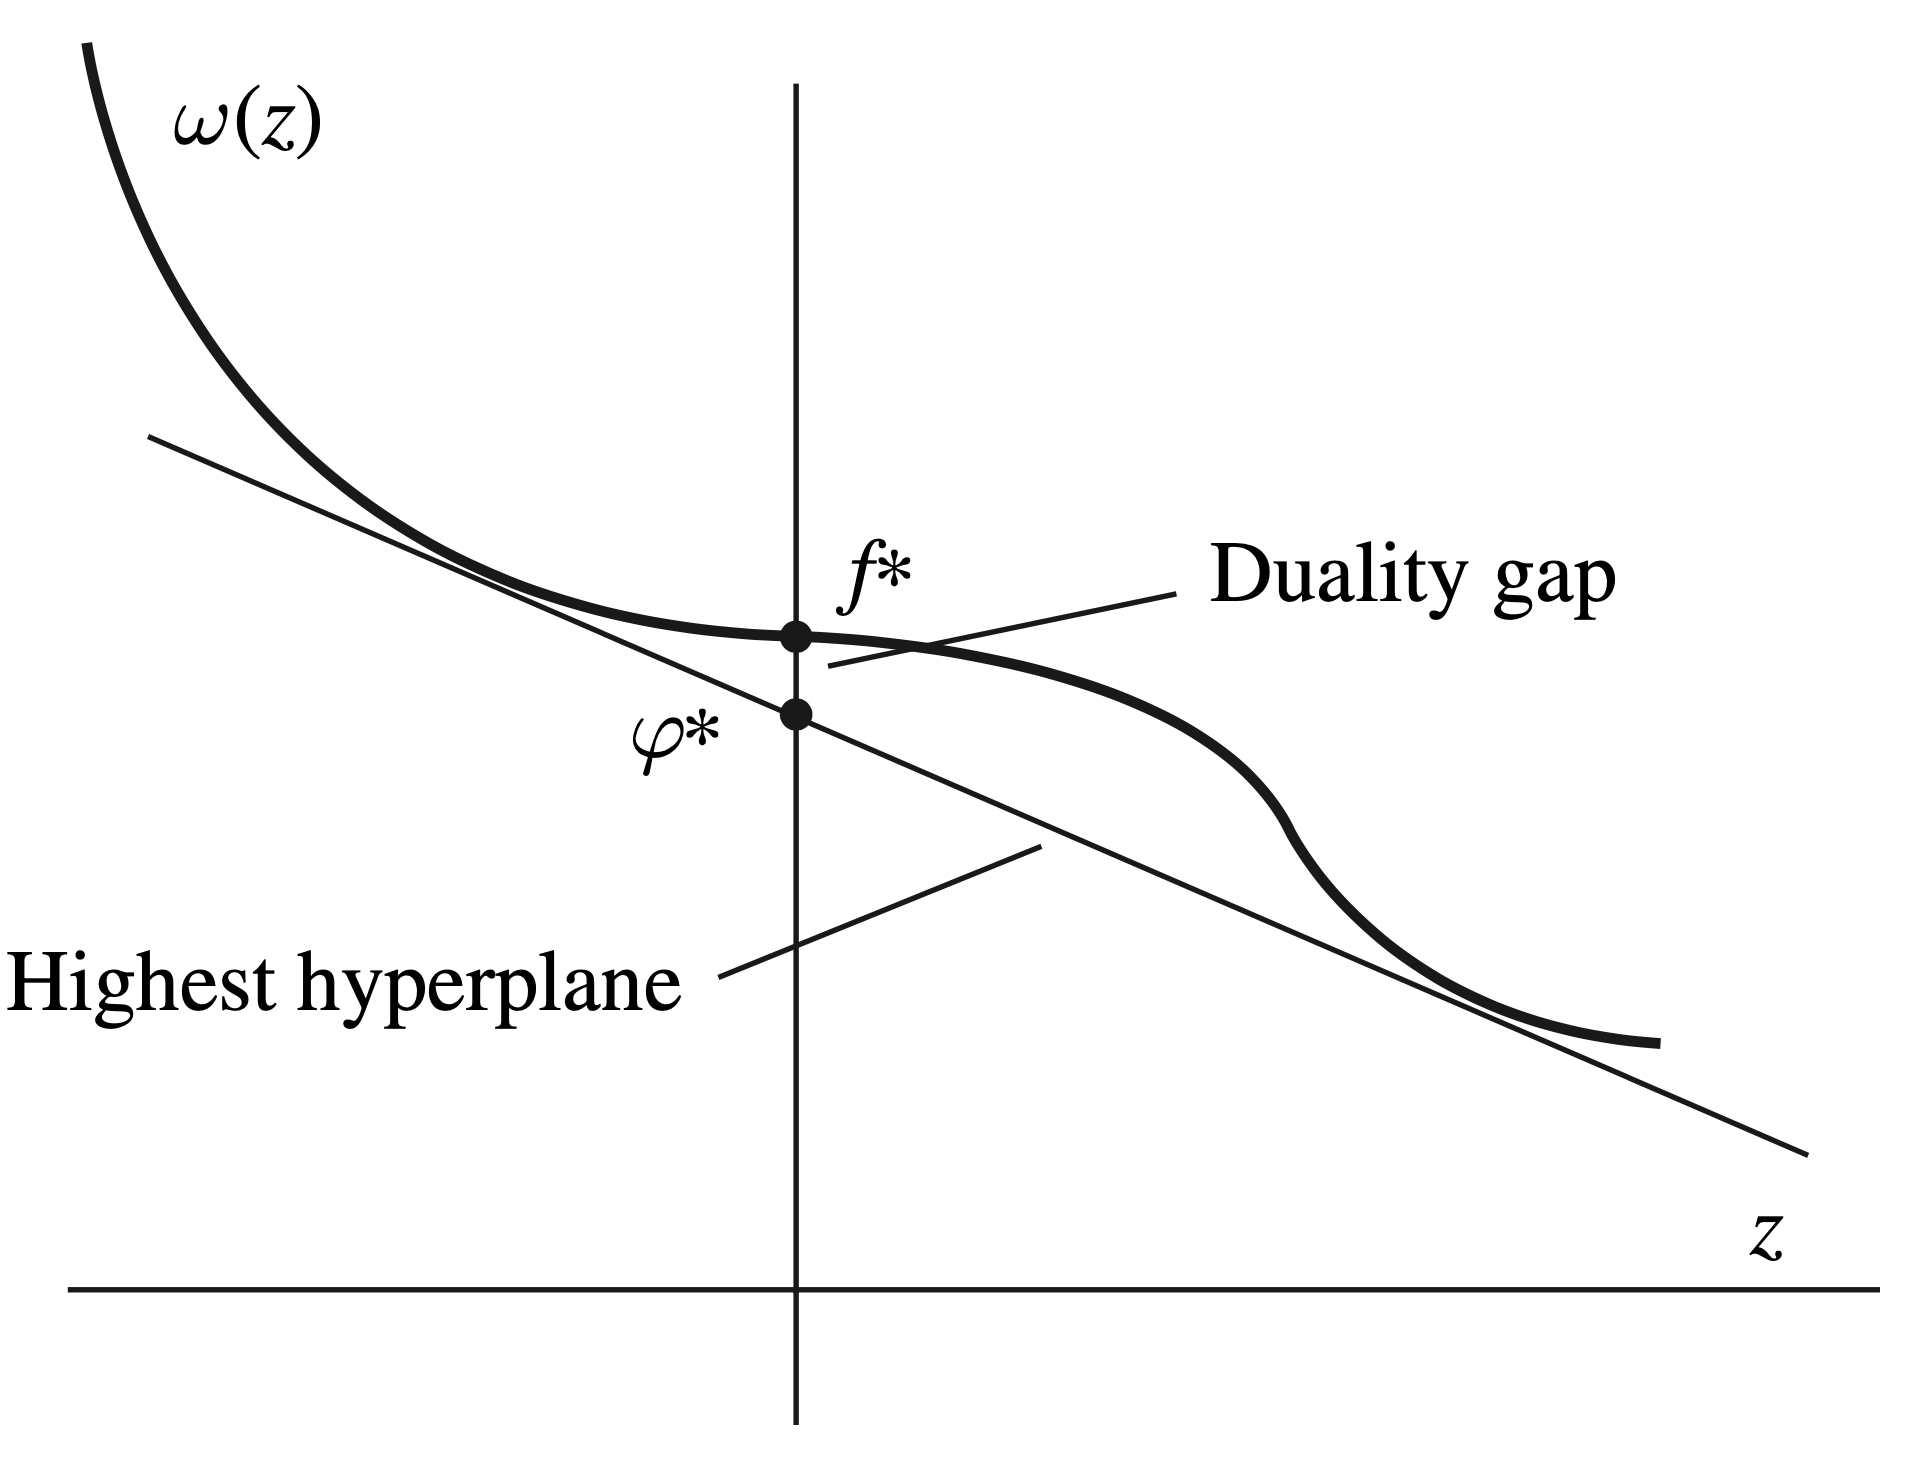
\includegraphics[scale=0.3]{\pref/highest-hyperplane.png}
    \caption{对偶间距的示意图.}
    \label{fig:highest-hyperplane}
\end{figure}

由此可以得到对偶性原理:位于$\omega$之下的超平面的最大截距等于刚刚碰到$\omega$的超平面的最小截距.

如果原始函数$\omega$是凸的,那么弱对偶定理可以被加强到强对偶定理,此时$\varphi^*$和$f^\ast$之间不再存在对偶间距,\Cref{fig:highest-hyperplane} 变成了\Cref{fig:strong-dual}.

\begin{figure}
    \centering
    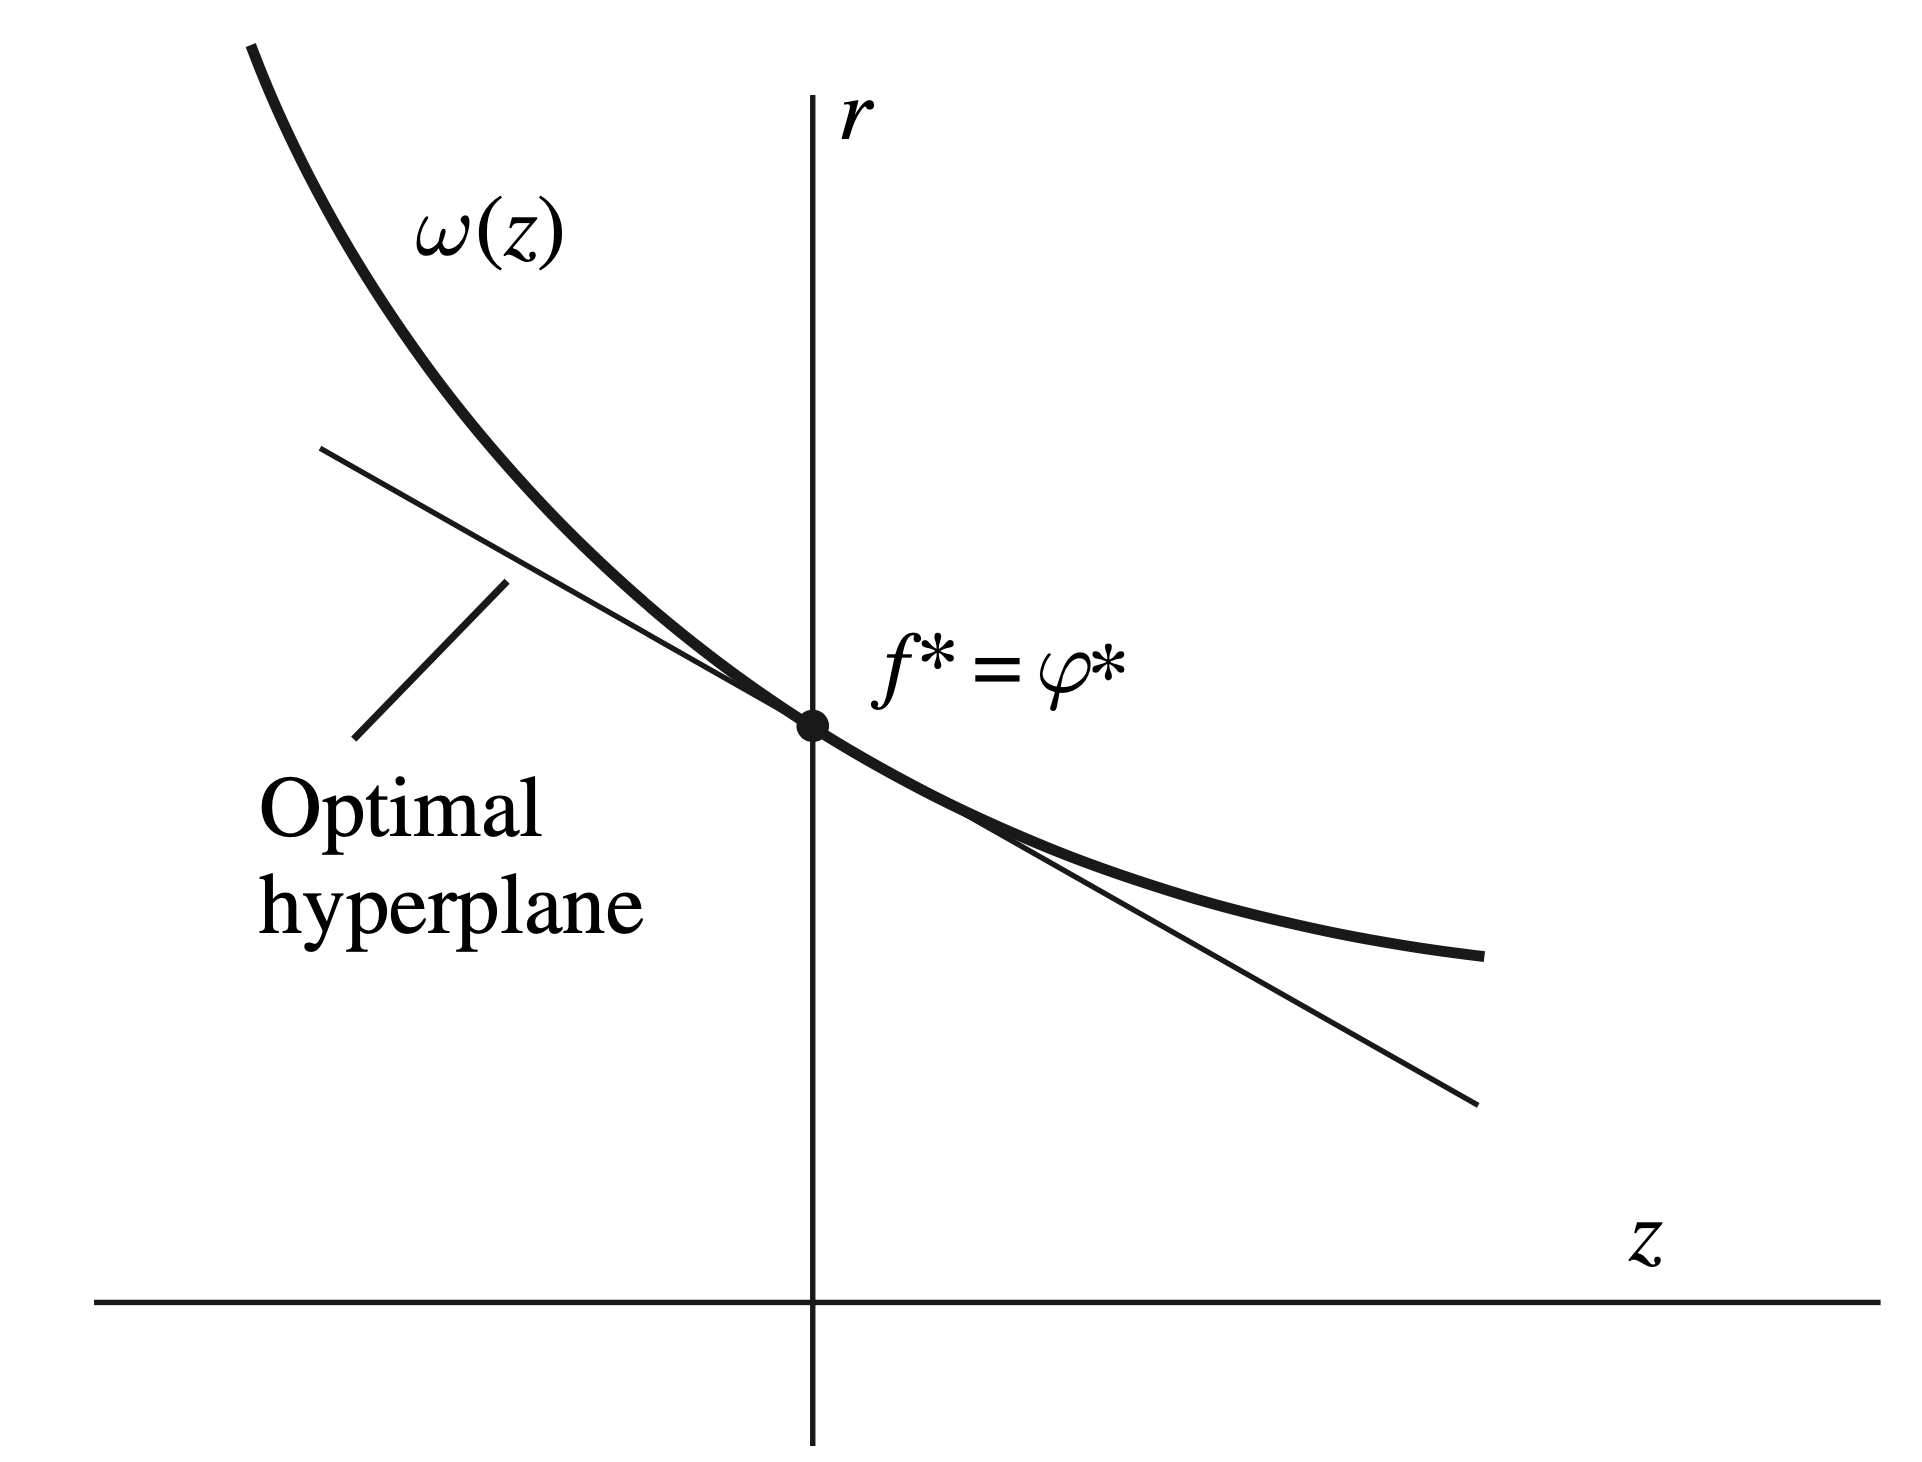
\includegraphics[scale=0.3]{\pref/strong-dual.png}
    \caption{强对偶定理的示意图.}
    \label{fig:strong-dual}
\end{figure}

下面我们叙述并证明强对偶定理. 我们直接考虑一般的优化问题.
\begin{equation}
        \begin{aligned}
    \min\quad & f({x}) \\
    \text{s.t.}\quad& {h(x)=0}, \\
    &g(x)\leq 0, \\
    &{x}\in\Omega.
    \end{aligned}\label{eq:mix-dual}
\end{equation}
其中,${h}$是$m$维仿射函数,${g}$是$p$维凸函数,$\Omega\subseteq\R^n$是凸集. 

原始函数\index{原始函数}可以写作
    \[\omega(y,z)=\inf\{f(x):\exists x\in\Omega\ h(x)=y, g(x)\leq z\}.\]
对偶函数\index{对偶函数}定义为:$$\varphi({\lambda,\mu})=\inf\{f({x})+{\lambda^\t h(x)+\mu^\t g(x):x}\in\Omega\}.$$
它的最大值记为
    $$\varphi^\ast=\sup\{\varphi({\lambda,\mu}):{\lambda}\in \R^m,{\mu}\in \R^p,{\mu}\ge {0}\}.$$

利用以上定义,我们可以表述强对偶定理如下:
\begin{theorem}[强对偶定理]
在问题 \eqref{eq:mix-dual} 中,假设${h}$是对于$\Omega$正规的,在可行域内$g$满足正规性条件. 假设${x^\ast}$是问题 \eqref{eq:mix-dual} 的解,设$f({x^\ast})=f^\ast$. 那么对每个${\lambda}$和${\mu}\ge{0}$都有
$$\varphi(\lambda,\mu)\le f^\ast.$$
另外,存在${\lambda,\mu\ge 0}$使得
$$\varphi({\lambda,\mu})=f^\ast.$$
因此$\varphi^\ast=f^\ast$. 与此同时,$\lambda,\mu$是该问题的Lagrange乘子.
\end{theorem} 

\begin{proof}
由Lagrange零阶条件定理(\Cref{thm:mix-zero-cond})可知:
    \begin{align*}
        f^\ast&=\min\{f({x})+{\lambda^\t h(x)+\mu^\t g(x):x}\in\Omega\}\\
        &=\varphi({\lambda,\mu})\le\varphi^\ast\le f^\ast.
    \end{align*}
因此,$\varphi^\ast=f^\ast$,并且取等号的$\lambda,\mu$是Lagrange乘子.
\end{proof}

从对偶原理我们可以写出对偶规划的一般形式:
    \begin{align*}
    \begin{array}{cc}
        \text{原始问题} &\qquad \text{对偶问题} \\
        \begin{aligned}
            \min\quad&\omega(y,z)\\
            \text{s.t.}\quad &y=0,\\
            &z\leq 0.
        \end{aligned}&\qquad
        \begin{aligned}
            \max\quad&\varphi(\lambda,\mu)\\
            \text{s.t.}\quad &\lambda\in\R^m,\\
            &\mu\geq 0.
        \end{aligned}
    \end{array}
    \end{align*}
作为例子,下面我们给一个对偶规划的经济学解释. 

\begin{example}[线性规划的经济学解释]
\Cref{tab:cleaner} 描述了公司甲用原料生产清洁剂的价格与存量表. 
\begin{table}
        \centering
        \begin{tabular}{c|ccc|c}
        \hline
                 & 原料1&原料2&原料3&售价(万元/吨) \\
                 \hline
             清洁剂A  & 0.25&0.50&0.25&12 \\
             清洁剂B & 0.50&0.50& &15\\
             \hline
             存量(吨)&120&150&50& \\
             \hline
        \end{tabular}
        \caption{清洁剂原料价格存量表. }
        \label{tab:cleaner}
\end{table}

甲用3种原料混合成2种清洁剂. 2种清洁剂应该如何配制,使总价值最大?

设清洁剂A和B分别配制$x_1$和$x_2$,我们可以把甲的目标写成一个规划问题:
\begin{align*}
\begin{array}{lrcl}
\max\quad&\multicolumn{3}{l}{z=12x_1+15x_2}\\
\text{s.t.}\quad&0.25x_1+0.50x_2&\le&120,\\
&0.50x_1+0.50x_2&\le&150,\\
&0.25x_1&\le& 50,\\
&x_1&\ge& 0,\\
&x_2&\ge& 0.
\end{array}
\end{align*}

现在有一个公司乙需要这3种原料,打算向甲购买,应付出多少钱?

乙向甲购买3种原料,出价分别为每吨$y_1,y_2,y_3$万元. 希望总价格尽量小,但不能低于甲用原料生产清洁剂所产生的价值,因此写出规划问题为:
\[
 \begin{array}{lrcl}
\min\quad&\multicolumn{3}{l}{w=120y_1+150y_2+50y_3} \\
\text{s.t.}\quad& 0.25y_1+0.50y_2+0.25y_3&\ge&12,\\
&0.50y_1+0.50y_2&\ge&15,\\
&y_1&\ge&0,\\
&y_2&\ge&0,\\
&y_3&\ge&0.
 \end{array}
\]
注意到,以上两个规划问题恰好互为对偶问题.
\end{example}

\section{应用:支持向量机(SVM)}\index{支持向量机}\index{SVM}

作为前面极值必要条件的一个具体应用,我们考虑一个经典的机器学习分类器:\emph{支持向量机}(SVM). 

考虑二分类问题,输入$x\in \R^n$,函数$f$输出一个$\{-1,1\}$中的值. 二分类问题的学习问题指的是给定训练集$\{(x_i,y_i)\}_{i=1}^N$,找到$f$使得$f(x_i)=y_i$. 假设训练集是线性可分的,例如,存在某个$w\in \R^n$和$b\in \R$使得
    $$f(x)=\begin{cases}
		1,& w^\t x+b>0,\\
		-1, &w^\t x+b<0.
	\end{cases}$$

学习问题的首要目标是找到正确的以及最优的$w$和$b$. 本质上说,这就是一个\emph{找分离超平面}\index{分离超平面}的过程. 那么,什么才叫最优呢?从几何视角来看,一个自然的想法是最大化\emph{分离距离}\index{分离距离},即训练集中所有点到分离超平面的距离和的最小值,见\Cref{fig:svm}.
\begin{figure}
    \centering
    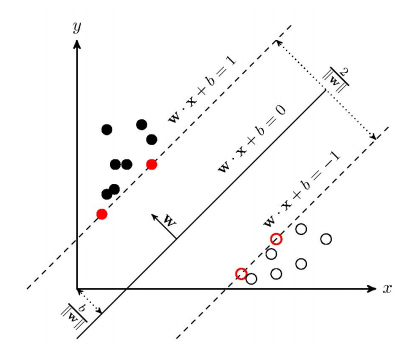
\includegraphics[scale=0.8]{\pref/svm.png}
    \caption{分离距离示意图.}
    \label{fig:svm}
\end{figure}

采样点$x_i$到分离超平面的归一化距离为
    $$\gamma_i=y_i\left(\left(\frac{w}{\norm{w}_2}\right)^\t x+\frac{b}{\norm{w}_2}\right).$$
$\gamma=\min_i\gamma_i$是最小的归一化距离. 于是我们的任务变成了最大化$\gamma$. 等价地,我们求解如下优化问题
\begin{align*}
    \max_{w,b}\quad&\gamma \\
    \text{s.t.}\quad&\gamma\le\gamma_i,\quad i=1,2,\dots,N.
\end{align*}

$\gamma\le\gamma_i$等价于$$y_i\left(\left(\frac{w}{\gamma\norm{w}_2}\right)^\t x+\frac{b}{\gamma\norm{w}_2}\right)\geq 1.$$
简洁起见,把$w$替换成$\frac{w}{\gamma\norm{w}_2}$,把$b$替换成$\frac{b}{\gamma\norm{w}_2}$,我们有$$y_i(w^\t x+b)\geq 1.$$
那么最大化$\gamma=\frac{1}{\norm{w}_2}$等价于最小化$\norm{w}_2^2$. 

我们得到以下凸规划问题:
\begin{align*}
    \min_{w,b}\quad&\frac{1}{2}\|w\|_2^2\\
    \text{s.t. }\quad &y_i(w^\t x_i+b)\geq 1,\quad i=1,2,\cdots, N.
\end{align*}

如何解决这个问题?利用上面的对偶理论,我们有如下步骤:
\begin{itemize}
    \item 第一步,用Lagrange乘子法,转化成Lagrange问题(min-max).
    \item 第二步,写出对偶问题(max-min),验证强对偶定理的正规性条件,于是只需要求解对偶规划.
    \item 第三步,写出KKT条件,将对偶规划解为一个二次规划(min) ,用优化算法求解二次规划.
\end{itemize}

\endgroup